% Metódy inžinierskej práce

\documentclass[10pt,twoside,slovak,a4paper]{article}

\usepackage[slovak]{babel}
%\usepackage[T1]{fontenc}
\usepackage[IL2]{fontenc} % lepšia sadzba písmena Ľ než v T1
\usepackage[utf8]{inputenc}
\usepackage{graphicx}
\usepackage{url} % príkaz \url na formátovanie URL
\usepackage{hyperref} % odkazy v texte budú aktívne (pri niektorých triedach dokumentov spôsobuje posun textu)

\usepackage{cite}
%\usepackage{times}



\title{Počítače v šachu \thanks{Semestrálny projekt v predmete Metódy inžinierskej práce, ak. rok 2022/23, vedenie: ing. Vladimír Mlynarovič PhD.}} % meno a priezvisko vyučujúceho na cvičeniach

\author{Martin Horský\\[2pt]
	{\small Slovenská technická univerzita v Bratislave}\\
	{\small Fakulta informatiky a informačných technológií}\\
	{\small \texttt{xhorskym1@stuba.sk}}
	}

\date{\small 27. september 2022}



\begin{document}

\maketitle

\begin{abstract}
Počítače uľahčujú náš život už niekoľko generácií. Umožňujú množstvo pokrokov v každej sfére každého priemyslu, aký si dokážeme predstaviť Výnimkou v tomto ohľade nie je ani šach. Prinášajú nám rôzne spôsoby zlepšovania našich schopností, oboznamujú nás s populárnymi stratégiami, ale taktiež nám umožňujú podvádzať. Okrem toho však aj prinášajú šach do verejného povedomia. Vďaka online šachu môžeme hrať šach s kýmkoľvek na svete bez toho, aby sme museli čo i len vlastniť šachovnicu. Vďaka médiám sa o šach mnohí ľudia, ktorým by nikdy ani neprišiel na um, začínajú zaujímať. Vďaka počítačom je dnes šach taký aký je.
\end{abstract}


\section{Úvod}\label{intro}

V časti šachové enginy\ref{enginy} je najprv opísaná história šachových enginov. Ďalej je vysvetlený pojem inexaktné problémy a metódy, akými sa riešia a spôsoby, ktorými sa využívajú priamo pri šachu. Následovne budú opísané najnovšie šachové enginy a na akom princípe fungujú. 
V časti šach online \ref{online} budú zas opísané stránky, pomocou ktorých môžme hrať šach cez internet. Potom v časti 4\ref{media} budú opísané spôsoby ktorými je šach popularizovaný v dnešnej dobe. A na koniec bude zhrnutie v časti 5\ref{zaver}

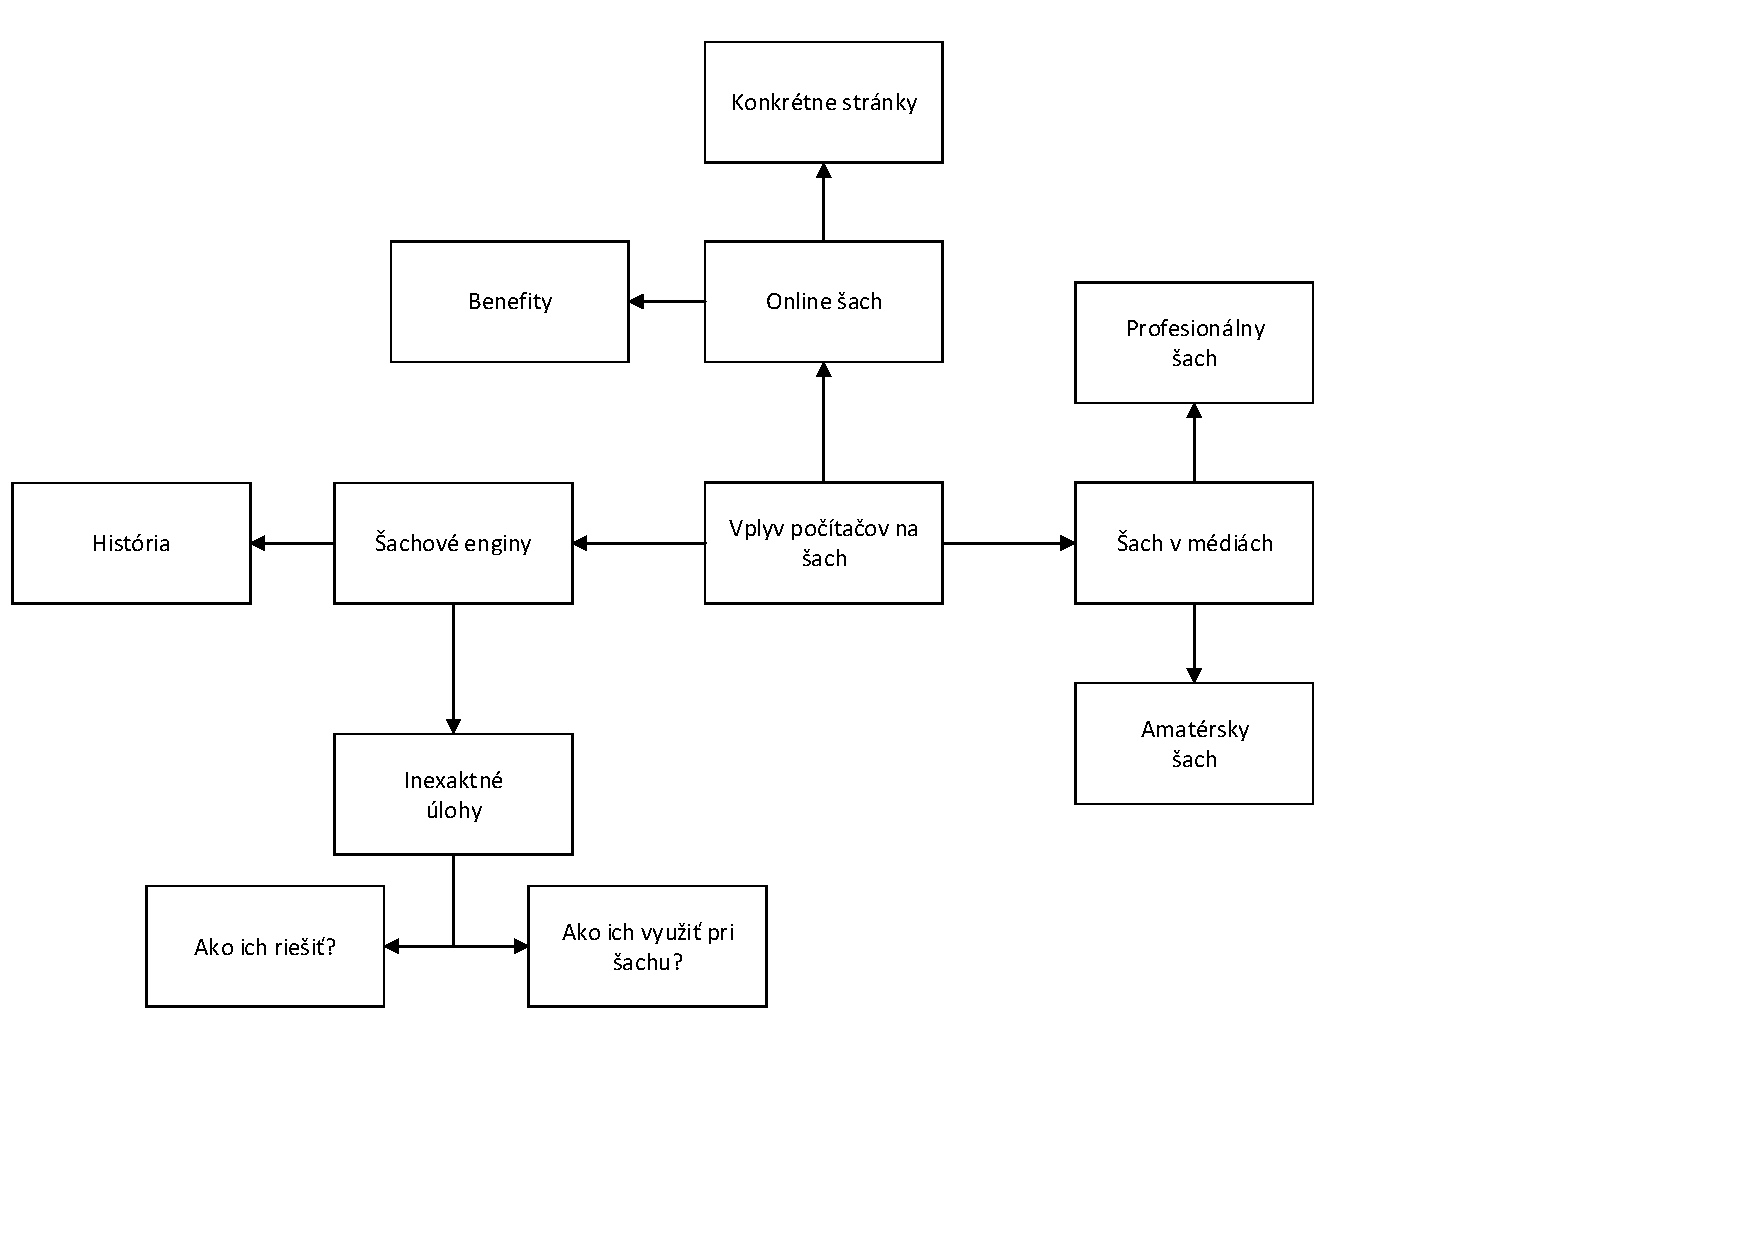
\includegraphics[scale=0.5]{mindmap}



\section{Šachové enginy} \label{enginy}
Šachové enginy sú počítače, ktoré podľa zložitých alogritmov hľadajú najlepší možný ťah, ktorý môže hráč zahrať.
\subsection{Historia šachových enginov} \label{enginy:historia}
Táto hra, mnohými považovaná za najvýznamnejšiu hru v histórii, má pôvod ešte pred 6. storočím v Indii, pod názvom Chatarunga. Postupom času, dôsledkom mnohých geopolitických vplyvov, sa v 10. storočí šach dostal až k nám do Európy nadobúdajúc nami známu formu v 15.storočí \cite{History-EB}. Počas nasledujúcich pár storočí, okrem pár zásahov pri priekopníkoch ako Ruy Lopez, sa stratégie príliš nemenili. Všetky hry pozostávali z pár naučených otváraní a pokračovali prevažne intuitívne. Túto situáciu zmenil príchod šachových enginov – počítačov určených na hľadanie najlepších možných ťahov.

Prvý „šachový engine“ vznikol už v roku 1769. Vynašiel ho Wolfgang von Kempelen, nazýval sa The Turk a mal dokonca aj hlasovú funkcionalitu. Nakoniec sa však ukázalo, že vo vnútri tohoto „počítača“ sa nachádzal človek, ktorý ťahy vykrikoval \cite{Levitt:Turk}. 

Pred dobou digitálnych počítačov existovalo ešte zopár počítačov, no v praxi neboli moc využiteľné. Slúžili len na vyriešenie veľmi špecifických situácií. Medzi tieto patril napríklad El Ajedrecista\cite{Williams:HODG}. Slúžil na vyriešenie situácie, kde zostali na doske len kráľ a veža proti kráľovi. Kvôli jednoduchému algoritmu sa mu vždy nepodarilo dať mat v čo najnižšom možnom počte ťahov, a často ani nie do 50 ťahov (čo by znamenalo remízu), ale vždy by dal mat a taktiež by detegoval ilegálny ťah protihráča. Odvtedy sa veľa šachových entuziastov, zručných v informačných technológiách, pokúšalo o napredovanie v tejto sfére. Jeden z mála šachových veľmajstrov (odteraz GM), ktorý tejto problematike venoval značnú snahu bol bývalý majster sveta Mikhail Botvinnik. Ten o tejto téme napísal množstvo kníh a taktiež slúžil ako konzultant pri vývoji programu týmu ITEP (Institute of Theoretical and Experimental Physics), ktorý bol výhercom prvého šachového zápasu medzi dvoma počítačmi. \cite{Botvinnik:CIC} 

V roku 1968 sa medzinárodný majster (odteraz IM) David Levy stavil, že ho najbližších 10 rokov nebude schopný žiadny engine poraziť. V roku 1978 túto stávku vyhral stavom 6-1, no činilo to prvú výhru počítača proti hráčovi na úrovni aspoň IM. \cite{LevyBet}

Postupne sa počítači stávali stále silnejšími protivníkmi. Špekulovalo sa kedy by sa počítač mohol stať svetovým šampiónom. Odborné odhady sa pohybovali všade od roku 1980 až po 2000. Tie optimistickejšie z nich sa nestali skutočnosťou, nakoľko vtedajší šampión, Gary Kasparov, bol porazený až ku koncu tohto odhadovaného obdobia, v roku 1997 \cite{Pandolfini:KasparovLoss}.

\subsection{Inexaktné úlohy} \label{enginy:inexactTask}
Čo sú to inexaktné úlohy? Rozhodovacie stromy môžu mať rôzne komplexity a rôzne veľkosti - malé, veľké alebo nekonečne veľké. Pri stromoch nekonečne veľkých alebo tak veľkých, že ich s našimi momentálnymi prostriedkami nedokážeme preskúmať musíme byť spokojní s inexaktnými, približnými, výsledkami. V prípade, že sú takéto nepresné výsledky prijateľné, snažíme sa eliminovať rozptyl variácií. Pri tejto metóde skracujeme rozhodovací strom. Čím viac je rozvetvený, tým bližšie ku koreňu musí byť skrátený. Ďalšia metóda je odrezávanie vetiev, u ktorých vidíme, že sa len vzďaľuje od cieľa. Ďalšou metódou je odrezávanie vetiev, pri ktorých vieme, že sa po niekoľkých krokoch dostanú k hodnote, ktorú iná vetva už nadobudla.

Ako to využiť v šachu? Profesionálni hráči využívajú pri hraní dve metódy. Prvou je, že si danú situáciu pamätajú z predošlých hier, ktoré buď odohrali alebo študovali. Druhou je, že si predstavia všetky zmysluplné ťahy a snažia sa nájsť najlepšie možné reakcie. Tieto si musia predstaviť na niekoľko ťahov dopredu. Takmer všetky enginy majú svoju knižnicu otváracích sekvencií, čo je v podstate využitie prvej metódy. Na druhú metódu sa pozerajú ako na inexaktné úlohy. Hľadajú všetky možné ťahy, pričom odstraňujú sekvencie ťahov, ktoré teoreticky nedávajú zmysel, tie čo by viedli k opakovaniu ťahov, alebo zbytočnému naťahovaniu a tie, čo by viedli k remíze alebo prehre. Engine má v tomto ohľade nevýhodu oproti človeku, čo sa týka efektivity, vzhľadom na to, že nevidí tak jasne, aký ťah dáva zmysel. No je to zároveń výhodné v situáciach, kde najlepší ťah spočíva v obetovaní svojej či už svojej pozície, alebo figúrky takým spôsobom, že to z počiatku pôsobí ako chyba, no vyvinie sa z toho brilantný ťah.

\subsection{Moderné enginy} \label{newEngines}
Najvyužívanejšími šachovým enginmi sú Stockfish a Leela. Používajú ich väčšina šachových aplikácií, ktoré sú verejne dostupné. Sú to open source programy. To znamená, že kódy týchto programov sú verejne dostupné a je povolené ich využitie na komerčné účely. 

Alpha Zero je šachový engine spoločnosti DeepMind, čo je dcérskou spoločnosťou Google. Momentálne má najvyššie ELO (hodnotenie na základe schopnosti v porovnaní s ostatnými). Oproti enginom Stockfish a Leela využíva taktiež GPU, čo zlepšuje výkonnosť. Tento engine nie je open source.

\section{Šach online} \label{online}

Umožnenie hrania šachu je kľúčovým faktorom jeho momentálnej popularity. Dôkazom toho je úspešnosť najpopulárnejšej webovej stránky na hranie šachu chess.com. Finančný zisk len z ich aplikácie činil v októbri 2022 odhadom 2 milióny dolárov\cite{ChessCom-Revenue}. V tejto sume nie sú zahrnuté zisky od PC uživateľov. Toto vysoké číslo nie je prekvapivé, vzhľadom na to, že mesačne má táto stránka 20 miliónov uživateľov. \cite{ChessCom-MonthlyUsers}. 

Táto stránka priťahuje toľkých uživateľov svojim prehľadným uživateľským prostredím, ale aj rôznymi módmi, kde je možné hrať šach s poupravenými pravidlami. Okrem hrania tiež ponúka prémiovým uživateľom rôzne lekcie sústrediacich sa na rôzne fázy hry. 

Ďalšie populárne stránky sú chess24 a lichess. Tie však neponúkajú toľko funkcionalít a nemajú tak dobré uživateľské prostredie a preto zaostávajú za chess.com. 

Stránke lichess však v poslednej dobe vysoko stúpla popularita, kvôli tomu, že svetový šampión Magnus Carlsen hral exkluzívne na tejto stránke. 



\section{Popularizácia šachu v digitálnych médiách} \label{media}

Možnosť hrania šachu online je síce skvelá, no sama o sebe, bez propagácie, by nemala takmer žiadny význam v popularizácii šachu. V tomto ohľade veľmi napomohol seriál Queen's Gambit. Hračkárstva uvádzali zvýšenie predaju šachových setov až o 1100\%\cite{PostQGSales}. Ďalej tomu napomohla aktivita streamerov na stránke twitch.tv. Väčšina najpopulárnejších tvorcov na tejto stránke zdieľalo svoje hry šachu (Prevažne na stránke chess.com. Viacero streamerov malo aj oficiálny kontrakt, že budú hrať exkluzívne na tejto stránke). Následne aj mnoho profesionálnych hráčov začalo streamovať na tejto stránke. Medzi najpopulárnejších z nich patria Hikaru Nakamura a Magnus Carlsen. Neskôr bol usporiadaný turnaj PogChamps. Bol to turnaj medzi streamermi a celebritami, ktorých na turnaj pripravovali šachoví profesionáli. Tento turnaj dosiahol 375 tisíc súčasných sledovateľov.\cite{Keener-Boom}.


\section{Záver} \label{zaver} 
Šach je už stáročia jednou z najpopulárnejších hier a vďaka jeho digitalizácií pravdepodobne ňou aj nadlho zostane.




\bibliography{literatura}
\bibliographystyle{plain} % prípadne alpha, abbrv alebo hociktorý iný
\end{document}
